\chapter{МОДЕЛИРОВАНИЕ ФУНКЦИОНАЛЬНОГО УЗЛА УПРАВЛЕНИЯ МАТРИЧНЫМ ДИСПЛЕЕМ}
\label{cha:lab4}
\section{Постановка задачи}	

Требуется разработать модель цифрового логического устройства объёме ПЛИС Spartan-3E XC3S500E4PQ208C, сочетающую в себе
функциональные узлы делителя частоты 1кГц, фильтра дребезга контактов
кнопки и конечного автомата генератора последовательности.

Цифровой узел должен выводить на матричный дисплей размером восемь строк на восемь столбцов шестнадцатеричную цифру, значение которой определяется данной таблицы истинности и вектор-функции (Таблица~\ref{tab:4func-vector}).




\begin{table}[h!]
	\centering
	\caption{Вектор-функция}
	\begin{tabular}{|c|c|c|c|c|c|c|c|c|c|c|c|c|c|c|c|}
		\hline
		F & E & D & C & B & A & 9 & 8 & 7 & 6 & 5 & 4 & 3 & 2 & 1 & 0 \\ \hline\hline
		0 & 4 & 4 & 8 & 3 & 0 & 7 & 2 & 2 & D & 7 & C & 5 & 2 & A & C \\ \hline
	\end{tabular}
	\label{tab:4func-vector}
\end{table}


Организовать на языке Verilog тестовый модуль, осуществляющий верификацию написанных модулей. Тестовое окружение должно моделировать работу устройства на частоте 1 МГц. Функциональные узлы делителя частоты и фильтра в тестировании могут не участвовать.



\section{Моделирование цифрового устройства}
Приступим к реализации модели цифрового узла. Приведем структурную схему синтезируемой части проекта (см. Рисунок~\ref{fig:struct-scheme}).


\begin{figure}[h!]
	\centering
	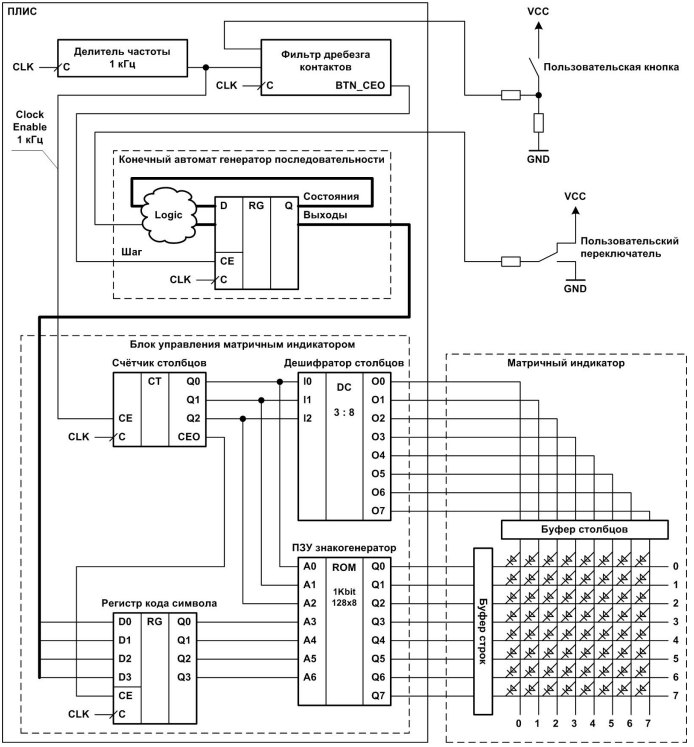
\includegraphics[width=0.6\linewidth]{course-plis/images/lab4/struct-scheme}
	\caption{Структурная схема синтезируемой части проекта}
	\label{fig:struct-scheme}
\end{figure}


Перечислим функциональные узлы, которые уже были реализованы ранее. 

\begin{enumerate}
	\item Делитель частоты. Реализован в разделе~\ref{cha:lab2}.
	\item Фильтр дребезга кнопок. Реализован в разделе~\ref{cha:lab2}.
	\item Конечный автомат генератор последовательности. Реализован в разделе~\ref{cha:lab2}.
\end{enumerate}

Процесс создания данных модулей не будет освещаться в настоящем разделе. 

\section{Принцип работы матричного индикатора}
Рассмотрим принцип работы матричного индикатора.
Вывод организуем по столбцам. В определённый момент времени активным является столбец,
и любые из восьми светодиодов активного столбца могут подсвечиваться
одновременно. 

Это даёт возможность увидеть одноцветное изображение,
выводимое на матричный дисплей, непосредственно на временной
диаграмме. Принцип вывода информации на матричный индикатор на
примере символа «9» показан на Рисунке~\ref{fig:display-principe}.

\begin{figure}[h!]
	\centering
	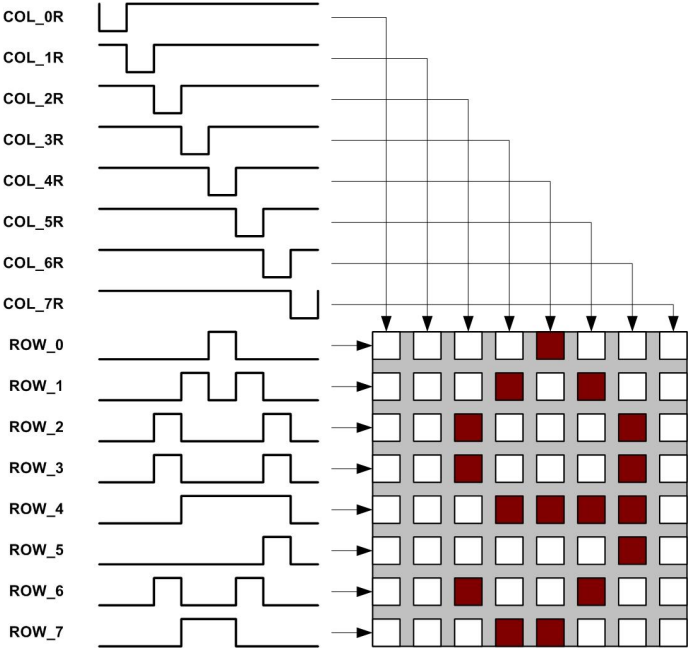
\includegraphics[width=0.5\linewidth]{course-plis/images/lab4/display-principe}
	\caption{Вывод символа на матричный индикатор}
	\label{fig:display-principe}
\end{figure}


\section{Создание проекта САПР Xilinx ISE}

\paragraph{Блок управления матричным индикатором}.
Была реализована модель функционального узла, выполняющего роль блока управления матричным дисплеем размеров восемь строк на восемь столбцов. Его работа организована по восходящему фронту синхросигнала CLK, сброс --- по восходящему фронту сигнала RST. 

Устройство содержит в себе счетчик столбцов, дешифратор столбцов, выбирающий в определенный момент времени только один активный столбец, а также элемент памяти (ПЗУ) хранящий шаблоны всех шестнадцатеричных чисел. ПЗУ будет использоваться знакогенератором для формирования символа из четырехразрядного двоичного входа, поданного в качестве входного сигнала.

Число шаблонов определяется числом символов и равно 16.
Объём ПЗУ знакогенератора составляет 1 кбит или 128 байт.

Младшие три разряда адреса ПЗУ выбирают текущий столбец в рамках
одного шаблона.
Старшие четыре разряда адреса ПЗУ выбирают текущий шаблон.

Шаблоны шестнадцатеричных чисел будут сформированы вручную и занесены в файл. В ходе моделирования работы устройства ПЗУ блока управления индикатором будет проинициализировано значениями, указанными в файле.

Исходный код данного функционального блока приведен в Приложении~\ref{cha:appendix1} в Листинге~\ref{lst:4lcd}.


\paragraph{Модуль верхнего уровня.}
Был описан модуль верхнего уровня, в которым подключены функциональные узлы моделируемого цифрового устройства согласно схеме, приведенной на Рисунке~\ref{fig:struct-scheme}.

В данном модуле использован делитель частоты DIV\_1MHz, преобразующий сигнал частотой 48МГц в сигнал частотой 1МГц.

Генератор последовательности fsm подключен к драйверу матричного дисплея lcd. Так текущее состояние автомата будет отображаться на матричном индикаторе.

Исходный код данного модуля приведен в Приложении~\ref{cha:appendix1} в Листинге~\ref{lst:4top}.

\paragraph{Тестовый модуль.}
Также был реализован модуль, который определяет тестовое окружение рассматриваемой части цифрового логического устройства. 

В модуле верхнего уровня описан генератор тактового сигнала частотой 48 МГц, использованный в качестве тактового сигнала для всех синхронных функциональных узлов в составе устройства. 

Сигнал с частотой 1МГц используется как сигнал разрешения счета для конечного автомата генератора последовательности, блока управления матричным индикатором, фильтра дребезга кнопок. 

Исходный код данного модуля приведен в Приложении~\ref{cha:appendix1} в Листинге~\ref{lst:4test-top}.


\section{Тестирование и отладка средствами симулятора iSim}
После компоновки проекта, подключения модуля верхнего уровня, была произведена верификация спроектированных моделей с помощью симулятора iSim из состава САПР Xilinx ISE Design Suite. Результаты тестирования можно видеть в Приложении~\ref{cha:appendix2} на Рисунках~\ref{fig:4isim}, на котором различимы повернутые на 180 градусов шестнадцатеричные числа, соответствующие исходной вектор-функции (см. Рисунок~\ref{tab:4func-vector}).


\section{Вывод}

В данном разделе нами были получены общие навыки работы с программным обеспечением Xilinx ISE Design Suite, изучены основы языка Verilog.

С помощью полученных знаний был спроектирован функциональный узел по управлению матричным индикатором, который был использован для вывода текущего состояния автомата--генератора последовательности.


